\documentclass[10pt,openany,a4paper]{article}
\usepackage{graphicx} 
\usepackage{multirow}
\usepackage{enumitem}
\usepackage{amssymb}
\usepackage{amsmath}
\usepackage{xcolor}
\usepackage{cancel}
\usepackage{tcolorbox}
\usepackage{geometry}
\usepackage{tikz, pgfplots, tkz-euclide,calc}
    \usetikzlibrary{patterns,snakes,shapes.arrows,3d}
	\geometry{
		total = {160mm, 237mm},
		left = 25mm,
		right = 35mm,
		top = 30mm,
		bottom = 30mm,
	}

\newcommand{\jawab}{\textbf{Jawab}:}

\begin{document}
    \pagenumbering{gobble}
    \begin{tabular}{|lcl|}
     \hline
     Nama&:&Teosofi Hidayah Agung\\
     NRP&:&5002221132\\
     \hline
    \end{tabular}\\~\\
    \textbf{Latihan A}
    \begin{enumerate}
        \setcounter{enumi}{7}
        \item Perlihatkan bahwa dengan persamaan parametrik $x=t\cos t,\,y=t\sin t,\,z=t$ terletak pada kerucut $z^2=x^2+y^2$. Gunakan fakta ini untuk membantu membuat sketsa kurva vektornya.\\
        \jawab\\
        Subtitusikan persamaan parametriknya, sehingga didapatkan
        \begin{flalign*}
            z^2&=x^2+y^2&\\
            t^2&=(t\cos t)^2+(t\sin t)^2&\\
            t^2&=t^2\cos^2 t+t^2\sin^2 t&\\
            t^2&=t^2(\cos^2 t+\sin^2 t)&\\
            t^2&=t^2\quad\blacksquare
        \end{flalign*}
        Sketsa grafiknya
        \begin{center}
            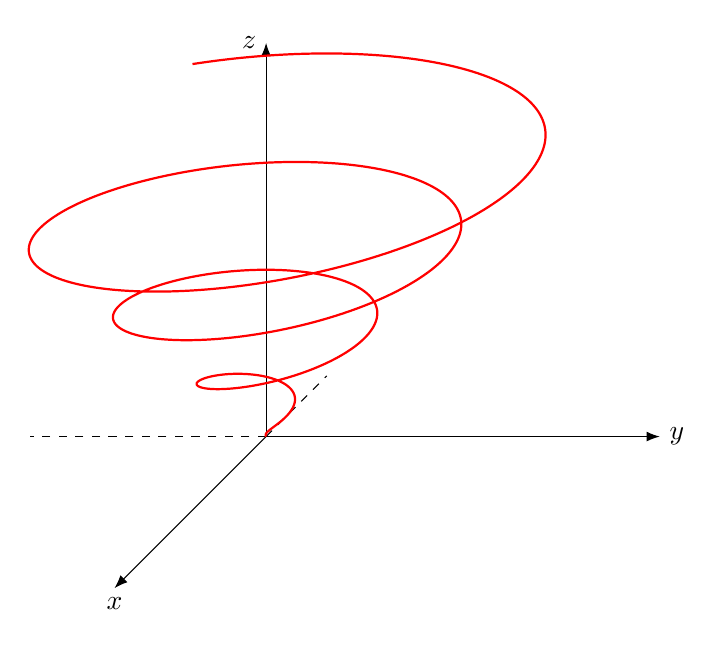
\begin{tikzpicture}[rotate around x=-90,rotate around y=0,rotate around z=-90]
                \draw[-Latex] (0,0,0) -- (5,0,0) node[below] {$x$};
                \draw[-Latex] (0,0,0) -- (0,5,0) node[right] {$y$};
                \draw[-Latex] (0,0,0) -- (0,0,5) node[left] {$z$};

                \draw[dashed] (0,0,0) -- (-2,0,0) node[below] {};
                \draw[dashed] (0,0,0) -- (0,-3,0) node[right] {};

                \draw[domain=0:3.6,samples = 1000,variable=\t,thick,red] plot({\t*cos(\t *360)},{\t*sin(\t *360)},{\t});
                
            \end{tikzpicture}
        \end{center}
        
        \item Perlihatkan bahwa dengan persamaan parametrik $x=\sin t,\,y=\cos t,\,z=\sin^2 t$ adalah kurva perpotongan dari permukaan $z=x^2$ dan $x^2+y^2=1$. Gunakan fakta ini untuk membantu membuat sketsa kurva vektornya.\\
        \jawab
        \begin{center}
            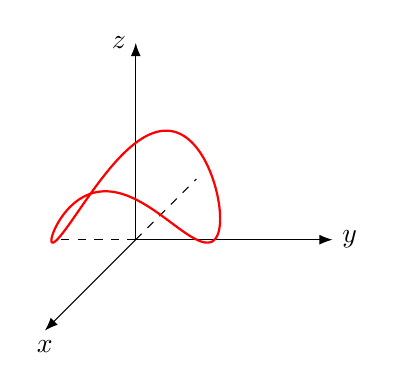
\begin{tikzpicture}[rotate around x=-90,rotate around y=0,rotate around z=-90]
                \draw[-Latex] (0,0,0) -- (3,0,0) node[below] {$x$};
                \draw[-Latex] (0,0,0) -- (0,2.5,0) node[right] {$y$};
                \draw[-Latex] (0,0,0) -- (0,0,2.5) node[left] {$z$};

                \draw[dashed] (0,0,0) -- (-2,0,0) node[below] {};
                \draw[dashed] (0,0,0) -- (0,-1,0) node[right] {};

                \draw[domain=0:3.6,samples = 1000,variable=\t,thick,red] plot({sin(\t *360)},{cos(\t *360)},{(sin(\t *360))^2});
            \end{tikzpicture}
        \end{center}
        
        \item Dapatkan fungsi vektor yang menyatakan kurva perpotongan dari kedua permukaan:
        \begin{enumerate}
            \item Silinder $x^2+y^2=4$ dan permukaan $z=xy$.\\
            \jawab
            \[x=2\cos t,\quad y=2\sin t,\quad z=(2\cos t)(2\sin t)=2\sin{2t}\]
            $\therefore\,r(t)=(2\cos t,2\sin t,2\sin{2t})$\\
            \item Kerucut $z=\sqrt{x^2+y^2}$ dan bidang $z=1+y$.\\
            \jawab
            \[x=\sqrt{2t+1},\quad y=t,\quad z=t+1\]
            $\therefore\,r(t)=(\sqrt{2t+1},t,t+1)$\\
            \item Parabolaida $z=4x^2+y^2$ dan silinder parabolik $y=x^2$.
            \[x=t,\quad y=t^2,\quad z=4t^2+t^4\]
            $\therefore\,r(t)=(t,t^2,4t^2+t^4)$\\
        \end{enumerate}
        \textbf{Latihan B}
        \begin{enumerate}
            \item[4.] Jika diketahui $u(t)=t\,\vec{i}+2t^2\,\vec{k},\,v(t)=t^3\,\vec{j}+t\,\vec{k},\,w(t)=\vec{i}+t\vec{j}+t^2\vec{k}$, dapatkan:
            \begin{enumerate}
                \item[b)] $[(u+2v)\cdot w]'$\\
                \jawab
                \begin{flalign*}
                    [(u+2v)\cdot w]'&=[((t,0,2t^2)+2(0,t^3,t))\cdot (1,t,t^2)]'&\\
                    &=[(t,2t^3,2t^2+2t)\cdot (1,t,t^2)]'&\\
                    &=[t+2t^4+2t^4+2t^3]'&\\
                    &=[4t^4+2t^3+t]'&\\
                    &=16t^3+6t^2+1&\\
                \end{flalign*}
                \item[c)] $[(u\times v)\times w]'$\\
                \jawab
                \begin{flalign*}
                    [(u\times v)\times w]'&=
                    \left[\begin{vmatrix}
                        \vec{i}&\vec{j}&\vec{k}\\
                        t&0&2t^2\\
                        0&t^3&t
                    \end{vmatrix}\times (1,t,t^2)\right]'&\\
                    &=[(-2t^5\vec{i}-t^2\vec{j}+t^4\vec{k})\times (1,t,t^2)]'&\\
                    &=\left[\begin{vmatrix}
                        \vec{i}&\vec{j}&\vec{k}\\
                        -2t^5&-t^2&t^4\\
                        1&t&t^2
                    \end{vmatrix}\right]'&\\
                    &=[(-t^4-t^5)\vec{i}+(2t^7+t^4)\vec{j}+(-2t^6+t^2)\vec{k}]'&\\
                    &=(-4t^3-5t^4)\vec{i}+(14t^6+4t^3)\vec{j}+(-12t^5+2t)\vec{k}
                \end{flalign*}
            \end{enumerate}
            \item[7.] Dapatkan unit vektor singgung pada kurva $x=t,\,y=t^2,\,z=t^3$ pada titik dimana $t=1$.\\
            \jawab
            \begin{flalign*}
                r(t)&=t\vec{i}+t^2\vec{j}+t^3\vec{k}&\\
                r'(t)&=\vec{i}+2t\vec{j}+3t^2\vec{k}&\\
                r'(1)&=\vec{i}+2\vec{j}+3\vec{k}
            \end{flalign*}
            \[\therefore\,T(t)=\frac{r'(1)}{||r'(1)||}=\frac{1}{\sqrt{14}}(\vec{i}+2\vec{j}+3\vec{k})\]
            
            \item[8.] Carilah vektor singgung satuan $T(t)$ di titik dengan nilai parameter $t$ yang diberikan:
            \begin{enumerate}
                \item[b)] $r(t)=t\,\vec{i}+2\sin t\,\vec{j}+3\cos t \,\vec{k},\, t=\frac{\pi}{6}$\\
                \jawab
                \begin{flalign*}
                    r'(t)&=\vec{i}+2\cos t\,\vec{j}-3\sin t \,\vec{k}&\\
                    r'\left(\frac{\pi}{6}\right)&=\vec{i}+\sqrt{3}\vec{j}-\frac{3}{2} \,\vec{k}
                \end{flalign*}
                \[\therefore\,T(t)=\frac{r'\left(\frac{\pi}{6}\right)}{\left|\left|r'\left(\frac{\pi}{6}\right)\right|\right|}=\frac{2}{\sqrt{5}}\left(\vec{i}+\sqrt{3}\vec{j}-\frac{3}{2} \,\vec{k}\right)\]
                
                \item[c)] $r(t)=e^{2t}\cos t\vec{i}+e^{2t}\sin t\vec{j}+e^{2t} \vec{k},\, t=\frac{\pi}{2}$\\
                \jawab
                \begin{flalign*}
                    r'(t)&=e^{2t}(2\cos t-\sin t)\vec{i}+e^{2t}(2\sin t+\cos t)\vec{j}+2e^{2t} \vec{k}&\\
                    r'\left(\frac{\pi}{2}\right)&=-e^{\pi}\vec{i}+2e^{\pi}\vec{j}-2e^{\pi}\vec{k}
                \end{flalign*}
                \[\therefore\,T(t)=\frac{r'\left(\frac{\pi}{2}\right)}{\left|\left|r'\left(\frac{\pi}{2}\right)\right|\right|}=\frac{1}{3e^{\pi}}(-e^{\pi}\vec{i}+2e^{\pi}\vec{j}-2e^{\pi}\vec{k})\]
            \end{enumerate}
            \item[9.] Tentukan unit vektor singgung di suatu titik pada kurva $x=t^2+1,\,y=4t-3,\,z=2t^2-6t$ pada saat $t=2$.\\
            \jawab
            \begin{flalign*}
                r(t)&=(t^2+1)\vec{i}+(4t-3)\vec{j}+(2t^2-6t)\vec{k}&\\
                r'(t)&=2t\vec{i}+4\vec{j}+(4t-6)\vec{k}&\\
                r'(2)&=4\vec{i}+4\vec{j}+2\vec{k}
            \end{flalign*}
            \[\therefore\,T(t)=\frac{r'(2)}{||r'(2)||}=\frac{1}{3}(4\vec{i}+4\vec{j}+2\vec{k})\]
        \end{enumerate}
    \end{enumerate}
\end{document}